% Options for packages loaded elsewhere
\PassOptionsToPackage{unicode}{hyperref}
\PassOptionsToPackage{hyphens}{url}
%
\documentclass[
]{article}
\usepackage{amsmath,amssymb}
\usepackage{lmodern}
\usepackage{iftex}
\ifPDFTeX
  \usepackage[T1]{fontenc}
  \usepackage[utf8]{inputenc}
  \usepackage{textcomp} % provide euro and other symbols
\else % if luatex or xetex
  \usepackage{unicode-math}
  \defaultfontfeatures{Scale=MatchLowercase}
  \defaultfontfeatures[\rmfamily]{Ligatures=TeX,Scale=1}
\fi
% Use upquote if available, for straight quotes in verbatim environments
\IfFileExists{upquote.sty}{\usepackage{upquote}}{}
\IfFileExists{microtype.sty}{% use microtype if available
  \usepackage[]{microtype}
  \UseMicrotypeSet[protrusion]{basicmath} % disable protrusion for tt fonts
}{}
\makeatletter
\@ifundefined{KOMAClassName}{% if non-KOMA class
  \IfFileExists{parskip.sty}{%
    \usepackage{parskip}
  }{% else
    \setlength{\parindent}{0pt}
    \setlength{\parskip}{6pt plus 2pt minus 1pt}}
}{% if KOMA class
  \KOMAoptions{parskip=half}}
\makeatother
\usepackage{xcolor}
\usepackage[margin=1in]{geometry}
\usepackage{color}
\usepackage{fancyvrb}
\newcommand{\VerbBar}{|}
\newcommand{\VERB}{\Verb[commandchars=\\\{\}]}
\DefineVerbatimEnvironment{Highlighting}{Verbatim}{commandchars=\\\{\}}
% Add ',fontsize=\small' for more characters per line
\usepackage{framed}
\definecolor{shadecolor}{RGB}{248,248,248}
\newenvironment{Shaded}{\begin{snugshade}}{\end{snugshade}}
\newcommand{\AlertTok}[1]{\textcolor[rgb]{0.94,0.16,0.16}{#1}}
\newcommand{\AnnotationTok}[1]{\textcolor[rgb]{0.56,0.35,0.01}{\textbf{\textit{#1}}}}
\newcommand{\AttributeTok}[1]{\textcolor[rgb]{0.77,0.63,0.00}{#1}}
\newcommand{\BaseNTok}[1]{\textcolor[rgb]{0.00,0.00,0.81}{#1}}
\newcommand{\BuiltInTok}[1]{#1}
\newcommand{\CharTok}[1]{\textcolor[rgb]{0.31,0.60,0.02}{#1}}
\newcommand{\CommentTok}[1]{\textcolor[rgb]{0.56,0.35,0.01}{\textit{#1}}}
\newcommand{\CommentVarTok}[1]{\textcolor[rgb]{0.56,0.35,0.01}{\textbf{\textit{#1}}}}
\newcommand{\ConstantTok}[1]{\textcolor[rgb]{0.00,0.00,0.00}{#1}}
\newcommand{\ControlFlowTok}[1]{\textcolor[rgb]{0.13,0.29,0.53}{\textbf{#1}}}
\newcommand{\DataTypeTok}[1]{\textcolor[rgb]{0.13,0.29,0.53}{#1}}
\newcommand{\DecValTok}[1]{\textcolor[rgb]{0.00,0.00,0.81}{#1}}
\newcommand{\DocumentationTok}[1]{\textcolor[rgb]{0.56,0.35,0.01}{\textbf{\textit{#1}}}}
\newcommand{\ErrorTok}[1]{\textcolor[rgb]{0.64,0.00,0.00}{\textbf{#1}}}
\newcommand{\ExtensionTok}[1]{#1}
\newcommand{\FloatTok}[1]{\textcolor[rgb]{0.00,0.00,0.81}{#1}}
\newcommand{\FunctionTok}[1]{\textcolor[rgb]{0.00,0.00,0.00}{#1}}
\newcommand{\ImportTok}[1]{#1}
\newcommand{\InformationTok}[1]{\textcolor[rgb]{0.56,0.35,0.01}{\textbf{\textit{#1}}}}
\newcommand{\KeywordTok}[1]{\textcolor[rgb]{0.13,0.29,0.53}{\textbf{#1}}}
\newcommand{\NormalTok}[1]{#1}
\newcommand{\OperatorTok}[1]{\textcolor[rgb]{0.81,0.36,0.00}{\textbf{#1}}}
\newcommand{\OtherTok}[1]{\textcolor[rgb]{0.56,0.35,0.01}{#1}}
\newcommand{\PreprocessorTok}[1]{\textcolor[rgb]{0.56,0.35,0.01}{\textit{#1}}}
\newcommand{\RegionMarkerTok}[1]{#1}
\newcommand{\SpecialCharTok}[1]{\textcolor[rgb]{0.00,0.00,0.00}{#1}}
\newcommand{\SpecialStringTok}[1]{\textcolor[rgb]{0.31,0.60,0.02}{#1}}
\newcommand{\StringTok}[1]{\textcolor[rgb]{0.31,0.60,0.02}{#1}}
\newcommand{\VariableTok}[1]{\textcolor[rgb]{0.00,0.00,0.00}{#1}}
\newcommand{\VerbatimStringTok}[1]{\textcolor[rgb]{0.31,0.60,0.02}{#1}}
\newcommand{\WarningTok}[1]{\textcolor[rgb]{0.56,0.35,0.01}{\textbf{\textit{#1}}}}
\usepackage{longtable,booktabs,array}
\usepackage{calc} % for calculating minipage widths
% Correct order of tables after \paragraph or \subparagraph
\usepackage{etoolbox}
\makeatletter
\patchcmd\longtable{\par}{\if@noskipsec\mbox{}\fi\par}{}{}
\makeatother
% Allow footnotes in longtable head/foot
\IfFileExists{footnotehyper.sty}{\usepackage{footnotehyper}}{\usepackage{footnote}}
\makesavenoteenv{longtable}
\usepackage{graphicx}
\makeatletter
\def\maxwidth{\ifdim\Gin@nat@width>\linewidth\linewidth\else\Gin@nat@width\fi}
\def\maxheight{\ifdim\Gin@nat@height>\textheight\textheight\else\Gin@nat@height\fi}
\makeatother
% Scale images if necessary, so that they will not overflow the page
% margins by default, and it is still possible to overwrite the defaults
% using explicit options in \includegraphics[width, height, ...]{}
\setkeys{Gin}{width=\maxwidth,height=\maxheight,keepaspectratio}
% Set default figure placement to htbp
\makeatletter
\def\fps@figure{htbp}
\makeatother
\setlength{\emergencystretch}{3em} % prevent overfull lines
\providecommand{\tightlist}{%
  \setlength{\itemsep}{0pt}\setlength{\parskip}{0pt}}
\setcounter{secnumdepth}{-\maxdimen} % remove section numbering
\ifLuaTeX
  \usepackage{selnolig}  % disable illegal ligatures
\fi
\IfFileExists{bookmark.sty}{\usepackage{bookmark}}{\usepackage{hyperref}}
\IfFileExists{xurl.sty}{\usepackage{xurl}}{} % add URL line breaks if available
\urlstyle{same} % disable monospaced font for URLs
\hypersetup{
  pdftitle={Final Project Notebook},
  pdfauthor={Ian Mbaya},
  hidelinks,
  pdfcreator={LaTeX via pandoc}}

\title{Final Project Notebook}
\author{Ian Mbaya}
\date{2024-03-12}

\begin{document}
\maketitle

\hypertarget{load-the-neccessary-libraries}{%
\subsection{Load the Neccessary
Libraries}\label{load-the-neccessary-libraries}}

\begin{Shaded}
\begin{Highlighting}[]
\FunctionTok{library}\NormalTok{(}\StringTok{\textquotesingle{}tidyverse\textquotesingle{}}\NormalTok{)}
\end{Highlighting}
\end{Shaded}

\begin{verbatim}
## -- Attaching core tidyverse packages ------------------------ tidyverse 2.0.0 --
## v dplyr     1.1.4     v readr     2.1.4
## v forcats   1.0.0     v stringr   1.5.0
## v ggplot2   3.4.2     v tibble    3.2.1
## v lubridate 1.9.2     v tidyr     1.3.0
## v purrr     1.0.1     
## -- Conflicts ------------------------------------------ tidyverse_conflicts() --
## x dplyr::filter() masks stats::filter()
## x dplyr::lag()    masks stats::lag()
## i Use the conflicted package (<http://conflicted.r-lib.org/>) to force all conflicts to become errors
\end{verbatim}

\begin{Shaded}
\begin{Highlighting}[]
\FunctionTok{library}\NormalTok{(}\StringTok{\textquotesingle{}tidymodels\textquotesingle{}}\NormalTok{)}
\end{Highlighting}
\end{Shaded}

\begin{verbatim}
## -- Attaching packages -------------------------------------- tidymodels 1.1.0 --
## v broom        1.0.5     v rsample      1.1.1
## v dials        1.2.0     v tune         1.1.1
## v infer        1.0.4     v workflows    1.1.3
## v modeldata    1.1.0     v workflowsets 1.0.1
## v parsnip      1.1.1     v yardstick    1.2.0
## v recipes      1.0.6     
## -- Conflicts ----------------------------------------- tidymodels_conflicts() --
## x scales::discard() masks purrr::discard()
## x dplyr::filter()   masks stats::filter()
## x recipes::fixed()  masks stringr::fixed()
## x dplyr::lag()      masks stats::lag()
## x yardstick::spec() masks readr::spec()
## x recipes::step()   masks stats::step()
## * Search for functions across packages at https://www.tidymodels.org/find/
\end{verbatim}

\begin{Shaded}
\begin{Highlighting}[]
\FunctionTok{library}\NormalTok{(}\StringTok{\textquotesingle{}caret\textquotesingle{}}\NormalTok{)}
\end{Highlighting}
\end{Shaded}

\begin{verbatim}
## Loading required package: lattice
## 
## Attaching package: 'caret'
## 
## The following objects are masked from 'package:yardstick':
## 
##     precision, recall, sensitivity, specificity
## 
## The following object is masked from 'package:purrr':
## 
##     lift
\end{verbatim}

\begin{Shaded}
\begin{Highlighting}[]
\FunctionTok{library}\NormalTok{(}\StringTok{\textquotesingle{}pROC\textquotesingle{}}\NormalTok{)}
\end{Highlighting}
\end{Shaded}

\begin{verbatim}
## Type 'citation("pROC")' for a citation.
## 
## Attaching package: 'pROC'
## 
## The following objects are masked from 'package:stats':
## 
##     cov, smooth, var
\end{verbatim}

\begin{Shaded}
\begin{Highlighting}[]
\FunctionTok{library}\NormalTok{(}\StringTok{\textquotesingle{}lubridate\textquotesingle{}}\NormalTok{)}
\end{Highlighting}
\end{Shaded}

\hypertarget{loading-the-data}{%
\section{Loading the Data}\label{loading-the-data}}

\begin{Shaded}
\begin{Highlighting}[]
\NormalTok{attacks }\OtherTok{\textless{}{-}} \FunctionTok{read.csv}\NormalTok{(}\StringTok{"data/CTU2.csv"}\NormalTok{, }\AttributeTok{sep =} \StringTok{"|"}\NormalTok{)}
\end{Highlighting}
\end{Shaded}

\hypertarget{explalatory-data-analysis}{%
\section{Explalatory Data Analysis}\label{explalatory-data-analysis}}

\hypertarget{take-a-glimpse-of-the-data}{%
\subsection{Take a Glimpse of the
Data}\label{take-a-glimpse-of-the-data}}

\begin{Shaded}
\begin{Highlighting}[]
\FunctionTok{glimpse}\NormalTok{(attacks)}
\end{Highlighting}
\end{Shaded}

\begin{verbatim}
## Rows: 156,103
## Columns: 23
## $ ts             <dbl> 1526756262, 1526756269, 1526756273, 1526756280, 1526756~
## $ uid            <chr> "C9YvmJ3zxtuqxWxLW5", "CGsZqZ3UiQexLzPRVb", "C0LkBW2VEa~
## $ id.orig_h      <chr> "192.168.2.5", "192.168.2.5", "192.168.2.5", "192.168.2~
## $ id.orig_p      <dbl> 38792, 38792, 38793, 38793, 38794, 38794, 38795, 38795,~
## $ id.resp_h      <chr> "200.168.87.203", "200.168.87.203", "200.168.87.203", "~
## $ id.resp_p      <dbl> 59353, 59353, 59353, 59353, 59353, 59353, 59353, 59353,~
## $ proto          <chr> "tcp", "tcp", "tcp", "tcp", "tcp", "tcp", "tcp", "tcp",~
## $ service        <chr> "-", "-", "-", "-", "-", "-", "-", "-", "-", "-", "-", ~
## $ duration       <chr> "2.998333", "-", "2.997182", "-", "2.996286", "-", "2.9~
## $ orig_bytes     <chr> "0", "-", "0", "-", "0", "-", "0", "-", "0", "-", "0", ~
## $ resp_bytes     <chr> "0", "-", "0", "-", "0", "-", "0", "-", "0", "-", "0", ~
## $ conn_state     <chr> "S0", "S0", "S0", "S0", "S0", "S0", "S0", "S0", "S0", "~
## $ local_orig     <chr> "-", "-", "-", "-", "-", "-", "-", "-", "-", "-", "-", ~
## $ local_resp     <chr> "-", "-", "-", "-", "-", "-", "-", "-", "-", "-", "-", ~
## $ missed_bytes   <dbl> 0, 0, 0, 0, 0, 0, 0, 0, 0, 0, 0, 0, 0, 0, 0, 0, 0, 0, 0~
## $ history        <chr> "S", "S", "S", "S", "S", "S", "S", "S", "S", "S", "S", ~
## $ orig_pkts      <dbl> 3, 1, 3, 1, 3, 1, 3, 1, 3, 1, 3, 1, 3, 1, 6, 6, 1, 3, 1~
## $ orig_ip_bytes  <dbl> 180, 60, 180, 60, 180, 60, 180, 60, 180, 60, 180, 60, 1~
## $ resp_pkts      <dbl> 0, 0, 0, 0, 0, 0, 0, 0, 0, 0, 0, 0, 0, 1, 6, 6, 0, 0, 0~
## $ resp_ip_bytes  <dbl> 0, 0, 0, 0, 0, 0, 0, 0, 0, 0, 0, 0, 0, 76, 456, 456, 0,~
## $ tunnel_parents <chr> "-", "-", "-", "-", "-", "-", "-", "-", "-", "-", "-", ~
## $ label          <chr> "Malicious", "Malicious", "Malicious", "Malicious", "Ma~
## $ detailed.label <chr> "PartOfAHorizontalPortScan", "PartOfAHorizontalPortScan~
\end{verbatim}

\hypertarget{create-a-data-dictionary}{%
\subsection{Create a Data Dictionary}\label{create-a-data-dictionary}}

\begin{Shaded}
\begin{Highlighting}[]
\CommentTok{\# Data Dictionary for Network Connection Data}
\NormalTok{data\_dictionary }\OtherTok{\textless{}{-}}\NormalTok{ tibble}\SpecialCharTok{::}\FunctionTok{tribble}\NormalTok{(}
  \SpecialCharTok{\textasciitilde{}}\NormalTok{Field\_Name,     }\SpecialCharTok{\textasciitilde{}}\NormalTok{Description,                                   }\SpecialCharTok{\textasciitilde{}}\NormalTok{Type,}
  \StringTok{"ts"}\NormalTok{,            }\StringTok{"The timestamp of the connection event."}\NormalTok{,      }\StringTok{"time"}\NormalTok{,}
  \StringTok{"uid"}\NormalTok{,           }\StringTok{"A unique identifier for the connection."}\NormalTok{,     }\StringTok{"string"}\NormalTok{,}
  \StringTok{"id.orig\_h"}\NormalTok{,     }\StringTok{"The source IP address."}\NormalTok{,                      }\StringTok{"addr"}\NormalTok{,}
  \StringTok{"id.orig\_p"}\NormalTok{,     }\StringTok{"The source port."}\NormalTok{,                            }\StringTok{"port"}\NormalTok{,}
  \StringTok{"id.resp\_h"}\NormalTok{,     }\StringTok{"The destination IP address."}\NormalTok{,                 }\StringTok{"addr"}\NormalTok{,}
  \StringTok{"id.resp\_p"}\NormalTok{,     }\StringTok{"The destination port."}\NormalTok{,                       }\StringTok{"port"}\NormalTok{,}
  \StringTok{"proto"}\NormalTok{,         }\StringTok{"The network protocol used (e.g., \textquotesingle{}tcp\textquotesingle{})."}\NormalTok{,    }\StringTok{"enum"}\NormalTok{,}
  \StringTok{"service"}\NormalTok{,       }\StringTok{"The service associated with the connection."}\NormalTok{, }\StringTok{"string"}\NormalTok{,}
  \StringTok{"duration"}\NormalTok{,      }\StringTok{"The duration of the connection."}\NormalTok{,             }\StringTok{"interval"}\NormalTok{,}
  \StringTok{"orig\_bytes"}\NormalTok{,    }\StringTok{"The number of bytes sent from the source to the destination."}\NormalTok{, }\StringTok{"count"}\NormalTok{,}
  \StringTok{"resp\_bytes"}\NormalTok{,    }\StringTok{"The number of bytes sent from the destination to the source."}\NormalTok{, }\StringTok{"count"}\NormalTok{,}
  \StringTok{"conn\_state"}\NormalTok{,    }\StringTok{"The state of the connection."}\NormalTok{,                }\StringTok{"string"}\NormalTok{,}
  \StringTok{"local\_orig"}\NormalTok{,    }\StringTok{"Indicates whether the connection is considered local or not."}\NormalTok{, }\StringTok{"bool"}\NormalTok{,}
  \StringTok{"local\_resp"}\NormalTok{,    }\StringTok{"Indicates whether the connection is considered local or not."}\NormalTok{, }\StringTok{"bool"}\NormalTok{,}
  \StringTok{"missed\_bytes"}\NormalTok{,  }\StringTok{"The number of missed bytes in the connection."}\NormalTok{, }\StringTok{"count"}\NormalTok{,}
  \StringTok{"history"}\NormalTok{,       }\StringTok{"A history of connection states."}\NormalTok{,             }\StringTok{"string"}\NormalTok{,}
  \StringTok{"orig\_pkts"}\NormalTok{,     }\StringTok{"The number of packets sent from the source to the destination."}\NormalTok{, }\StringTok{"count"}\NormalTok{,}
  \StringTok{"orig\_ip\_bytes"}\NormalTok{, }\StringTok{"The number of IP bytes sent from the source to the destination."}\NormalTok{, }\StringTok{"count"}\NormalTok{,}
  \StringTok{"resp\_pkts"}\NormalTok{,     }\StringTok{"The number of packets sent from the destination to the source."}\NormalTok{, }\StringTok{"count"}\NormalTok{,}
  \StringTok{"resp\_ip\_bytes"}\NormalTok{, }\StringTok{"The number of IP bytes sent from the destination to the source."}\NormalTok{, }\StringTok{"count"}\NormalTok{,}
  \StringTok{"tunnel\_parents"}\NormalTok{,}\StringTok{"Indicates if this connection is part of a tunnel."}\NormalTok{, }\StringTok{"set[string]"}\NormalTok{,}
  \StringTok{"label"}\NormalTok{,         }\StringTok{"A label associated with the connection (e.g., \textquotesingle{}Malicious\textquotesingle{} or \textquotesingle{}Benign\textquotesingle{})."}\NormalTok{, }\StringTok{"string"}\NormalTok{,}
  \StringTok{"detailed\_label"}\NormalTok{,}\StringTok{"A more detailed description or label for the connection."}\NormalTok{, }\StringTok{"string"}
\NormalTok{)}

\CommentTok{\# Print the data dictionary}
\FunctionTok{print}\NormalTok{(data\_dictionary)}
\end{Highlighting}
\end{Shaded}

\begin{verbatim}
## # A tibble: 23 x 3
##    Field_Name Description                                                  Type 
##    <chr>      <chr>                                                        <chr>
##  1 ts         The timestamp of the connection event.                       time 
##  2 uid        A unique identifier for the connection.                      stri~
##  3 id.orig_h  The source IP address.                                       addr 
##  4 id.orig_p  The source port.                                             port 
##  5 id.resp_h  The destination IP address.                                  addr 
##  6 id.resp_p  The destination port.                                        port 
##  7 proto      The network protocol used (e.g., 'tcp').                     enum 
##  8 service    The service associated with the connection.                  stri~
##  9 duration   The duration of the connection.                              inte~
## 10 orig_bytes The number of bytes sent from the source to the destination. count
## # i 13 more rows
\end{verbatim}

\hypertarget{checking-for-missing-values}{%
\subsection{Checking for Missing
Values}\label{checking-for-missing-values}}

\begin{Shaded}
\begin{Highlighting}[]
\NormalTok{skimr}\SpecialCharTok{::}\FunctionTok{skim}\NormalTok{(attacks)}
\end{Highlighting}
\end{Shaded}

\begin{longtable}[]{@{}ll@{}}
\caption{Data summary}\tabularnewline
\toprule()
\endhead
Name & attacks \\
Number of rows & 156103 \\
Number of columns & 23 \\
\_\_\_\_\_\_\_\_\_\_\_\_\_\_\_\_\_\_\_\_\_\_\_ & \\
Column type frequency: & \\
character & 15 \\
numeric & 8 \\
\_\_\_\_\_\_\_\_\_\_\_\_\_\_\_\_\_\_\_\_\_\_\_\_ & \\
Group variables & None \\
\bottomrule()
\end{longtable}

\textbf{Variable type: character}

\begin{longtable}[]{@{}
  >{\raggedright\arraybackslash}p{(\columnwidth - 14\tabcolsep) * \real{0.2055}}
  >{\raggedleft\arraybackslash}p{(\columnwidth - 14\tabcolsep) * \real{0.1370}}
  >{\raggedleft\arraybackslash}p{(\columnwidth - 14\tabcolsep) * \real{0.1918}}
  >{\raggedleft\arraybackslash}p{(\columnwidth - 14\tabcolsep) * \real{0.0548}}
  >{\raggedleft\arraybackslash}p{(\columnwidth - 14\tabcolsep) * \real{0.0548}}
  >{\raggedleft\arraybackslash}p{(\columnwidth - 14\tabcolsep) * \real{0.0822}}
  >{\raggedleft\arraybackslash}p{(\columnwidth - 14\tabcolsep) * \real{0.1233}}
  >{\raggedleft\arraybackslash}p{(\columnwidth - 14\tabcolsep) * \real{0.1507}}@{}}
\toprule()
\begin{minipage}[b]{\linewidth}\raggedright
skim\_variable
\end{minipage} & \begin{minipage}[b]{\linewidth}\raggedleft
n\_missing
\end{minipage} & \begin{minipage}[b]{\linewidth}\raggedleft
complete\_rate
\end{minipage} & \begin{minipage}[b]{\linewidth}\raggedleft
min
\end{minipage} & \begin{minipage}[b]{\linewidth}\raggedleft
max
\end{minipage} & \begin{minipage}[b]{\linewidth}\raggedleft
empty
\end{minipage} & \begin{minipage}[b]{\linewidth}\raggedleft
n\_unique
\end{minipage} & \begin{minipage}[b]{\linewidth}\raggedleft
whitespace
\end{minipage} \\
\midrule()
\endhead
uid & 0 & 1 & 15 & 18 & 0 & 156103 & 0 \\
id.orig\_h & 0 & 1 & 9 & 15 & 0 & 961 & 0 \\
id.resp\_h & 0 & 1 & 9 & 15 & 0 & 64194 & 0 \\
proto & 0 & 1 & 3 & 4 & 0 & 3 & 0 \\
service & 0 & 1 & 1 & 4 & 0 & 5 & 0 \\
duration & 0 & 1 & 1 & 12 & 0 & 20105 & 0 \\
orig\_bytes & 0 & 1 & 1 & 4 & 0 & 48 & 0 \\
resp\_bytes & 0 & 1 & 1 & 4 & 0 & 137 & 0 \\
conn\_state & 0 & 1 & 2 & 5 & 0 & 11 & 0 \\
local\_orig & 0 & 1 & 1 & 1 & 0 & 1 & 0 \\
local\_resp & 0 & 1 & 1 & 1 & 0 & 1 & 0 \\
history & 0 & 1 & 1 & 11 & 0 & 68 & 0 \\
tunnel\_parents & 0 & 1 & 1 & 1 & 0 & 1 & 0 \\
label & 0 & 1 & 6 & 9 & 0 & 2 & 0 \\
detailed.label & 0 & 1 & 1 & 25 & 0 & 4 & 0 \\
\bottomrule()
\end{longtable}

\textbf{Variable type: numeric}

\begin{longtable}[]{@{}
  >{\raggedright\arraybackslash}p{(\columnwidth - 20\tabcolsep) * \real{0.1157}}
  >{\raggedleft\arraybackslash}p{(\columnwidth - 20\tabcolsep) * \real{0.0826}}
  >{\raggedleft\arraybackslash}p{(\columnwidth - 20\tabcolsep) * \real{0.1157}}
  >{\raggedleft\arraybackslash}p{(\columnwidth - 20\tabcolsep) * \real{0.1074}}
  >{\raggedleft\arraybackslash}p{(\columnwidth - 20\tabcolsep) * \real{0.0744}}
  >{\raggedleft\arraybackslash}p{(\columnwidth - 20\tabcolsep) * \real{0.0909}}
  >{\raggedleft\arraybackslash}p{(\columnwidth - 20\tabcolsep) * \real{0.0909}}
  >{\raggedleft\arraybackslash}p{(\columnwidth - 20\tabcolsep) * \real{0.0909}}
  >{\raggedleft\arraybackslash}p{(\columnwidth - 20\tabcolsep) * \real{0.0909}}
  >{\raggedleft\arraybackslash}p{(\columnwidth - 20\tabcolsep) * \real{0.0909}}
  >{\raggedright\arraybackslash}p{(\columnwidth - 20\tabcolsep) * \real{0.0496}}@{}}
\toprule()
\begin{minipage}[b]{\linewidth}\raggedright
skim\_variable
\end{minipage} & \begin{minipage}[b]{\linewidth}\raggedleft
n\_missing
\end{minipage} & \begin{minipage}[b]{\linewidth}\raggedleft
complete\_rate
\end{minipage} & \begin{minipage}[b]{\linewidth}\raggedleft
mean
\end{minipage} & \begin{minipage}[b]{\linewidth}\raggedleft
sd
\end{minipage} & \begin{minipage}[b]{\linewidth}\raggedleft
p0
\end{minipage} & \begin{minipage}[b]{\linewidth}\raggedleft
p25
\end{minipage} & \begin{minipage}[b]{\linewidth}\raggedleft
p50
\end{minipage} & \begin{minipage}[b]{\linewidth}\raggedleft
p75
\end{minipage} & \begin{minipage}[b]{\linewidth}\raggedleft
p100
\end{minipage} & \begin{minipage}[b]{\linewidth}\raggedright
hist
\end{minipage} \\
\midrule()
\endhead
ts & 0 & 1 & 1.526821e+09 & 37273.51 & 1526756240 & 1526788466 &
1526822257 & 1526853001 & 1526886287 & ▇▇▇▇▇ \\
id.orig\_p & 0 & 1 & 4.630844e+04 & 9667.61 & 3 & 39440 & 46810 & 53891
& 61530 & ▁▁▃▇▇ \\
id.resp\_p & 0 & 1 & 8.876350e+03 & 21140.31 & 0 & 22 & 22 & 22 & 59353
& ▇▁▁▁▂ \\
missed\_bytes & 0 & 1 & 0.000000e+00 & 0.00 & 0 & 0 & 0 & 0 & 0 &
▁▁▇▁▁ \\
orig\_pkts & 0 & 1 & 2.490000e+00 & 8.33 & 0 & 1 & 3 & 3 & 3031 &
▇▁▁▁▁ \\
orig\_ip\_bytes & 0 & 1 & 1.674000e+02 & 492.76 & 0 & 60 & 180 & 180 &
164117 & ▇▁▁▁▁ \\
resp\_pkts & 0 & 1 & 6.600000e-01 & 15.87 & 0 & 0 & 0 & 0 & 5975 &
▇▁▁▁▁ \\
resp\_ip\_bytes & 0 & 1 & 1.066000e+02 & 922.63 & 0 & 0 & 0 & 0 & 289732
& ▇▁▁▁▁ \\
\bottomrule()
\end{longtable}

\hypertarget{data-summary}{%
\section{Data Summary}\label{data-summary}}

\begin{Shaded}
\begin{Highlighting}[]
\FunctionTok{summary}\NormalTok{(attacks)}
\end{Highlighting}
\end{Shaded}

\begin{verbatim}
##        ts                uid             id.orig_h           id.orig_p    
##  Min.   :1.527e+09   Length:156103      Length:156103      Min.   :    3  
##  1st Qu.:1.527e+09   Class :character   Class :character   1st Qu.:39440  
##  Median :1.527e+09   Mode  :character   Mode  :character   Median :46810  
##  Mean   :1.527e+09                                         Mean   :46308  
##  3rd Qu.:1.527e+09                                         3rd Qu.:53891  
##  Max.   :1.527e+09                                         Max.   :61530  
##   id.resp_h           id.resp_p        proto             service         
##  Length:156103      Min.   :    0   Length:156103      Length:156103     
##  Class :character   1st Qu.:   22   Class :character   Class :character  
##  Mode  :character   Median :   22   Mode  :character   Mode  :character  
##                     Mean   : 8876                                        
##                     3rd Qu.:   22                                        
##                     Max.   :59353                                        
##    duration          orig_bytes         resp_bytes         conn_state       
##  Length:156103      Length:156103      Length:156103      Length:156103     
##  Class :character   Class :character   Class :character   Class :character  
##  Mode  :character   Mode  :character   Mode  :character   Mode  :character  
##                                                                             
##                                                                             
##                                                                             
##   local_orig         local_resp         missed_bytes   history         
##  Length:156103      Length:156103      Min.   :0     Length:156103     
##  Class :character   Class :character   1st Qu.:0     Class :character  
##  Mode  :character   Mode  :character   Median :0     Mode  :character  
##                                        Mean   :0                       
##                                        3rd Qu.:0                       
##                                        Max.   :0                       
##    orig_pkts        orig_ip_bytes        resp_pkts       resp_ip_bytes     
##  Min.   :   0.000   Min.   :     0.0   Min.   :   0.00   Min.   :     0.0  
##  1st Qu.:   1.000   1st Qu.:    60.0   1st Qu.:   0.00   1st Qu.:     0.0  
##  Median :   3.000   Median :   180.0   Median :   0.00   Median :     0.0  
##  Mean   :   2.488   Mean   :   167.4   Mean   :   0.66   Mean   :   106.6  
##  3rd Qu.:   3.000   3rd Qu.:   180.0   3rd Qu.:   0.00   3rd Qu.:     0.0  
##  Max.   :3031.000   Max.   :164117.0   Max.   :5975.00   Max.   :289732.0  
##  tunnel_parents        label           detailed.label    
##  Length:156103      Length:156103      Length:156103     
##  Class :character   Class :character   Class :character  
##  Mode  :character   Mode  :character   Mode  :character  
##                                                          
##                                                          
## 
\end{verbatim}

From the summary above it seems like we might have too many variables
that may not be contributing to the model. In the following steps we
will be reducing dimensionality by removing someof the columns

\hypertarget{dimensionality-reduction}{%
\subsection{Dimensionality Reduction}\label{dimensionality-reduction}}

\begin{Shaded}
\begin{Highlighting}[]
\CommentTok{\# Removing some of the less  important variables from the data }
\NormalTok{data1 }\OtherTok{\textless{}{-}} \FunctionTok{select}\NormalTok{(attacks, }
\NormalTok{                        label, ts,}
\NormalTok{                        id.orig\_h, id.resp\_h, }
\NormalTok{                        id.orig\_p, id.resp\_p, }
\NormalTok{                        proto, }
\NormalTok{                        conn\_state, duration, }
\NormalTok{                        resp\_ip\_bytes, orig\_ip\_bytes)}

\CommentTok{\# View the first few rows of the selected data}
\FunctionTok{summary}\NormalTok{(data1)}
\end{Highlighting}
\end{Shaded}

\begin{verbatim}
##     label                 ts             id.orig_h          id.resp_h        
##  Length:156103      Min.   :1.527e+09   Length:156103      Length:156103     
##  Class :character   1st Qu.:1.527e+09   Class :character   Class :character  
##  Mode  :character   Median :1.527e+09   Mode  :character   Mode  :character  
##                     Mean   :1.527e+09                                        
##                     3rd Qu.:1.527e+09                                        
##                     Max.   :1.527e+09                                        
##    id.orig_p       id.resp_p        proto            conn_state       
##  Min.   :    3   Min.   :    0   Length:156103      Length:156103     
##  1st Qu.:39440   1st Qu.:   22   Class :character   Class :character  
##  Median :46810   Median :   22   Mode  :character   Mode  :character  
##  Mean   :46308   Mean   : 8876                                        
##  3rd Qu.:53891   3rd Qu.:   22                                        
##  Max.   :61530   Max.   :59353                                        
##    duration         resp_ip_bytes      orig_ip_bytes     
##  Length:156103      Min.   :     0.0   Min.   :     0.0  
##  Class :character   1st Qu.:     0.0   1st Qu.:    60.0  
##  Mode  :character   Median :     0.0   Median :   180.0  
##                     Mean   :   106.6   Mean   :   167.4  
##                     3rd Qu.:     0.0   3rd Qu.:   180.0  
##                     Max.   :289732.0   Max.   :164117.0
\end{verbatim}

\hypertarget{visualizing-pattern-in-network-traffic-based-on-timestamps}{%
\subsection{Visualizing Pattern in Network Traffic based on
Timestamps}\label{visualizing-pattern-in-network-traffic-based-on-timestamps}}

\begin{Shaded}
\begin{Highlighting}[]
\CommentTok{\# Convert \textquotesingle{}ts\textquotesingle{} to a DateTime object }
\NormalTok{data1}\SpecialCharTok{$}\NormalTok{ts }\OtherTok{\textless{}{-}} \FunctionTok{as.POSIXct}\NormalTok{(data1}\SpecialCharTok{$}\NormalTok{ts, }\AttributeTok{format =} \StringTok{"\%Y{-}\%m{-}\%d \%H:\%M:\%S"}\NormalTok{)  }

\CommentTok{\# Create a new dataframe with counts of attacks per time period (e.g., per day)}
\NormalTok{attacks\_per\_period }\OtherTok{\textless{}{-}}\NormalTok{ data1 }\SpecialCharTok{\%\textgreater{}\%}
  \FunctionTok{group\_by}\NormalTok{(}\AttributeTok{ts =} \FunctionTok{floor\_date}\NormalTok{(ts, }\StringTok{"day"}\NormalTok{), label) }\SpecialCharTok{\%\textgreater{}\%}  \CommentTok{\# group by day and label;  }
  \FunctionTok{summarise}\NormalTok{(}\AttributeTok{count =} \FunctionTok{n}\NormalTok{(), }\AttributeTok{.groups =} \StringTok{\textquotesingle{}drop\textquotesingle{}}\NormalTok{)  }\CommentTok{\# count the number of rows (attacks) per group}

\CommentTok{\# Create the time series plot}
\FunctionTok{ggplot}\NormalTok{(attacks\_per\_period, }\FunctionTok{aes}\NormalTok{(}\AttributeTok{x =}\NormalTok{ ts, }\AttributeTok{y =}\NormalTok{ count, }\AttributeTok{group =}\NormalTok{ label, }\AttributeTok{color =}\NormalTok{ label)) }\SpecialCharTok{+}
  \FunctionTok{geom\_line}\NormalTok{() }\SpecialCharTok{+}  
  \FunctionTok{labs}\NormalTok{(}\AttributeTok{title =} \StringTok{"Time Series of Attacks"}\NormalTok{, }\AttributeTok{x =} \StringTok{"Time"}\NormalTok{, }\AttributeTok{y =} \StringTok{"Count of Attacks"}\NormalTok{, }\AttributeTok{color =} \StringTok{"Label"}\NormalTok{) }\SpecialCharTok{+}
  \FunctionTok{theme\_minimal}\NormalTok{() }\SpecialCharTok{+}
  \FunctionTok{scale\_x\_datetime}\NormalTok{(}\AttributeTok{date\_breaks =} \StringTok{"1 day"}\NormalTok{, }\AttributeTok{date\_labels =} \StringTok{"\%b \%d"}\NormalTok{)  }
\end{Highlighting}
\end{Shaded}

\includegraphics{Notebook_files/figure-latex/unnamed-chunk-5-1.pdf}

\hypertarget{exploring-the-categorical-variables}{%
\subsection{Exploring The Categorical
Variables}\label{exploring-the-categorical-variables}}

\begin{Shaded}
\begin{Highlighting}[]
\CommentTok{\# First lets Calculate the count of unique values}
\NormalTok{unique\_counts }\OtherTok{\textless{}{-}}\NormalTok{ attacks }\SpecialCharTok{\%\textgreater{}\%}
  \FunctionTok{summarise}\NormalTok{(}
    \AttributeTok{unique\_id\_orig\_h =} \FunctionTok{n\_distinct}\NormalTok{(id.orig\_h),}
    \AttributeTok{unique\_id\_resp\_h =} \FunctionTok{n\_distinct}\NormalTok{(id.resp\_h),}
    \AttributeTok{unique\_id\_orig\_p =} \FunctionTok{n\_distinct}\NormalTok{(id.orig\_p),}
    \AttributeTok{unique\_id\_resp\_p =} \FunctionTok{n\_distinct}\NormalTok{(id.resp\_p),}
    \AttributeTok{unique\_proto =} \FunctionTok{n\_distinct}\NormalTok{(proto),}
    \AttributeTok{unique\_conn\_state =} \FunctionTok{n\_distinct}\NormalTok{(conn\_state)}
\NormalTok{  )}

\CommentTok{\# Print the unique counts}
\FunctionTok{print}\NormalTok{(unique\_counts)}
\end{Highlighting}
\end{Shaded}

\begin{verbatim}
##   unique_id_orig_h unique_id_resp_h unique_id_orig_p unique_id_resp_p
## 1              961            64194            26740               11
##   unique_proto unique_conn_state
## 1            3                11
\end{verbatim}

\#\#Visualizing Three Categorical Variables on a Barchart

\begin{Shaded}
\begin{Highlighting}[]
\CommentTok{\# Ensure all varaibales are factors}
\NormalTok{attacks}\SpecialCharTok{$}\NormalTok{label }\OtherTok{\textless{}{-}} \FunctionTok{as.factor}\NormalTok{(attacks}\SpecialCharTok{$}\NormalTok{label)}
\NormalTok{attacks}\SpecialCharTok{$}\NormalTok{proto }\OtherTok{\textless{}{-}} \FunctionTok{as.factor}\NormalTok{(attacks}\SpecialCharTok{$}\NormalTok{proto)}
\NormalTok{attacks}\SpecialCharTok{$}\NormalTok{conn\_state }\OtherTok{\textless{}{-}} \FunctionTok{as.factor}\NormalTok{(attacks}\SpecialCharTok{$}\NormalTok{conn\_state)}
\NormalTok{attacks}\SpecialCharTok{$}\NormalTok{id.resp\_p}\OtherTok{\textless{}{-}} \FunctionTok{as.factor}\NormalTok{(attacks}\SpecialCharTok{$}\NormalTok{id.resp\_p)}

\CommentTok{\# Plot1 Protocols}
\FunctionTok{ggplot}\NormalTok{(}\AttributeTok{data =}\NormalTok{ attacks, }\FunctionTok{aes}\NormalTok{(}\AttributeTok{x =}\NormalTok{ proto, }\AttributeTok{fill =}\NormalTok{ label)) }\SpecialCharTok{+}
  \FunctionTok{geom\_bar}\NormalTok{(}\AttributeTok{position =} \StringTok{"dodge"}\NormalTok{) }\SpecialCharTok{+}
  \FunctionTok{labs}\NormalTok{(}\AttributeTok{title =} \StringTok{"Distribution of Labels across Protocols"}\NormalTok{,}
       \AttributeTok{x =} \StringTok{"Protocols"}\NormalTok{,}
       \AttributeTok{y =} \StringTok{"Count"}\NormalTok{) }\SpecialCharTok{+}
  \FunctionTok{scale\_fill\_brewer}\NormalTok{(}\AttributeTok{palette =} \StringTok{"Set1"}\NormalTok{)  }\CommentTok{\# This changes the color palette}
\end{Highlighting}
\end{Shaded}

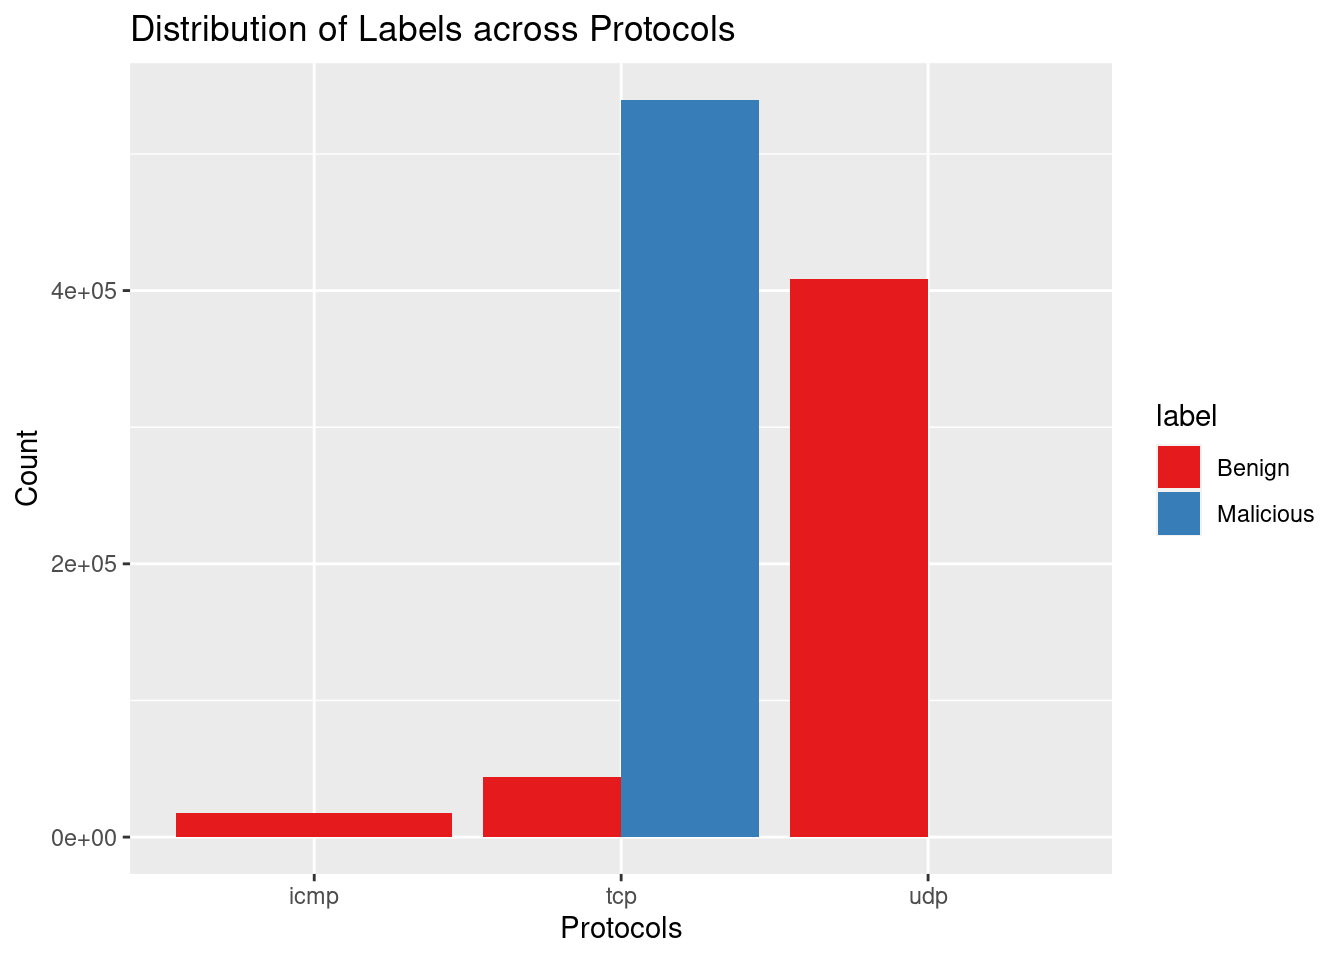
\includegraphics{Notebook_files/figure-latex/categorical-viz-1.pdf}

\begin{Shaded}
\begin{Highlighting}[]
\CommentTok{\# Plot2 Connection State}
\FunctionTok{ggplot}\NormalTok{(}\AttributeTok{data =}\NormalTok{ attacks, }\FunctionTok{aes}\NormalTok{(}\AttributeTok{x =}\NormalTok{ conn\_state, }\AttributeTok{fill =}\NormalTok{ label)) }\SpecialCharTok{+}
  \FunctionTok{geom\_bar}\NormalTok{(}\AttributeTok{position =} \StringTok{"dodge"}\NormalTok{) }\SpecialCharTok{+}
  \FunctionTok{labs}\NormalTok{(}\AttributeTok{title =} \StringTok{"Distribution of Labels across Connection States"}\NormalTok{,}
       \AttributeTok{x =} \StringTok{"Connection State"}\NormalTok{,}
       \AttributeTok{y =} \StringTok{"Count"}\NormalTok{) }\SpecialCharTok{+}
  \FunctionTok{scale\_fill\_brewer}\NormalTok{(}\AttributeTok{palette =} \StringTok{"Set1"}\NormalTok{)  }\CommentTok{\# This changes the color palette}
\end{Highlighting}
\end{Shaded}

\includegraphics{Notebook_files/figure-latex/categorical-viz-2.pdf}

\begin{Shaded}
\begin{Highlighting}[]
\CommentTok{\# Plot3 Destination pR}
\FunctionTok{ggplot}\NormalTok{(}\AttributeTok{data =}\NormalTok{ attacks, }\FunctionTok{aes}\NormalTok{(}\AttributeTok{x =}\NormalTok{ id.resp\_p, }\AttributeTok{fill =}\NormalTok{ label)) }\SpecialCharTok{+}
  \FunctionTok{geom\_bar}\NormalTok{(}\AttributeTok{position =} \StringTok{"dodge"}\NormalTok{) }\SpecialCharTok{+}
  \FunctionTok{labs}\NormalTok{(}\AttributeTok{title =} \StringTok{"Distribution of Labels across Destination Port"}\NormalTok{,}
       \AttributeTok{x =} \StringTok{"Connection State"}\NormalTok{,}
       \AttributeTok{y =} \StringTok{"Count"}\NormalTok{) }\SpecialCharTok{+}
  \FunctionTok{scale\_fill\_brewer}\NormalTok{(}\AttributeTok{palette =} \StringTok{"Set1"}\NormalTok{)  }\CommentTok{\# This changes the color palette}
\end{Highlighting}
\end{Shaded}

\includegraphics{Notebook_files/figure-latex/categorical-viz-3.pdf}
\#\#Exploring the Numeric Variables

\begin{Shaded}
\begin{Highlighting}[]
\NormalTok{resp.ip\_gt\_zero }\OtherTok{\textless{}{-}} \FunctionTok{sum}\NormalTok{(data1}\SpecialCharTok{$}\NormalTok{resp\_ip\_bytes }\SpecialCharTok{\textgreater{}} \DecValTok{0}\NormalTok{)}

\NormalTok{orig.ip\_gt\_180 }\OtherTok{\textless{}{-}} \FunctionTok{sum}\NormalTok{(data1}\SpecialCharTok{$}\NormalTok{resp\_ip\_bytes }\SpecialCharTok{\textgreater{}} \DecValTok{180}\NormalTok{)}

\NormalTok{null\_durations }\OtherTok{\textless{}{-}} \FunctionTok{sum}\NormalTok{(data1}\SpecialCharTok{$}\NormalTok{duration }\SpecialCharTok{==} \StringTok{"{-}"}\NormalTok{)}
\end{Highlighting}
\end{Shaded}

\hypertarget{separating-data-into-train-and-test}{%
\subsection{Separating Data into Train and
Test}\label{separating-data-into-train-and-test}}

\begin{Shaded}
\begin{Highlighting}[]
\CommentTok{\# Create a data partition}
\FunctionTok{set.seed}\NormalTok{(}\DecValTok{5774}\NormalTok{)  }
\NormalTok{trainIndex }\OtherTok{\textless{}{-}} \FunctionTok{createDataPartition}\NormalTok{(data1}\SpecialCharTok{$}\NormalTok{label, }\AttributeTok{p =} \FloatTok{0.8}\NormalTok{, }\AttributeTok{list =} \ConstantTok{FALSE}\NormalTok{, }\AttributeTok{times =} \DecValTok{1}\NormalTok{)}

\CommentTok{\# Create training and test datasets}
\NormalTok{train }\OtherTok{\textless{}{-}}\NormalTok{ data1[trainIndex, ]}
\NormalTok{test }\OtherTok{\textless{}{-}}\NormalTok{ data1[}\SpecialCharTok{{-}}\NormalTok{trainIndex, ]}

\CommentTok{\# Viewing the dimensions of the train and test sets}
\FunctionTok{dim}\NormalTok{(train)}
\end{Highlighting}
\end{Shaded}

\begin{verbatim}
## [1] 124883     11
\end{verbatim}

\begin{Shaded}
\begin{Highlighting}[]
\FunctionTok{dim}\NormalTok{(test)}
\end{Highlighting}
\end{Shaded}

\begin{verbatim}
## [1] 31220    11
\end{verbatim}

\hypertarget{building-and-training-the-logistic-regression-model}{%
\subsection{Building and Training The Logistic Regression
Model}\label{building-and-training-the-logistic-regression-model}}

\hypertarget{testing-model-and-cross-validation}{%
\subsection{Testing Model and Cross
Validation}\label{testing-model-and-cross-validation}}

\hypertarget{results-and-model-intepretation}{%
\subsection{Results and Model
Intepretation}\label{results-and-model-intepretation}}

\end{document}
